Pipelines are critical for safe and efficient transportation of fluids across long distances.  For example, pipelines are used by utility companies to transport clean water and natural gas to homes for heating and living purposes.  Furthermore, pipelines are also used in agriculture to transport irrigation water to hydrate crops.  Moreover, pipelines are used by energy companies for transporting energy-rich hydrocarbons to fuel the world's transportation and manufacturing. In the United States, over 70\% of petroleum products are shipped by pipeline.  In Canada, the number increases to 97\% \cite{pipeline_transport}.  The latest data in 2014 estimates that there are about 3,500,000 km of operational pipelines in 120 countries \cite{CIA_pipeline}. Due to the world's dependency on pipelines for transporting their basic needs, ensuring its reliability and efficiency has a global-scale impact.

Typical pipelines have hundreds of digital measurements per minute and are hard to analyze; however, machine learning methods benefit greatly from large amounts of data. Thus, an opportunity was discovered where machine learning methods will be applied to pipelines used to transport petroleum products. The objectives of this project were to leverage machine learning to identify anomalous pipeline behaviour, and to build a real time optimization tool.

In this chapter, a time-series neural network classifier will first be introduced to detect anomalous activity within any pipeline equipment.  Then, a real time optimization tool based on a linear model optimized using mixed integer linear program will be introduced.  Due to confidentiality agreements, all data presented here-forth will be normalized, and all parties of this project will remain anomalous.

\section{Process Introduction}
Two separate pipelines, Line 11 and Line RM06A, were analyzed.  Line 11 is a simplistic pipeline; data from line 11 were used to build an anomaly detection tool.  Line RM06A was more complex; therefore, a real time optimization (RTO) tool was build for this line.

\subsection{Line 11}
The schematic of line 11 is shown in Figure \ref{fig:08Line11}. For Line 11, the objective was to build an anomaly detection tool for unexpected shut downs of its pumps.  

\begin{figure}[h]
    \centering
    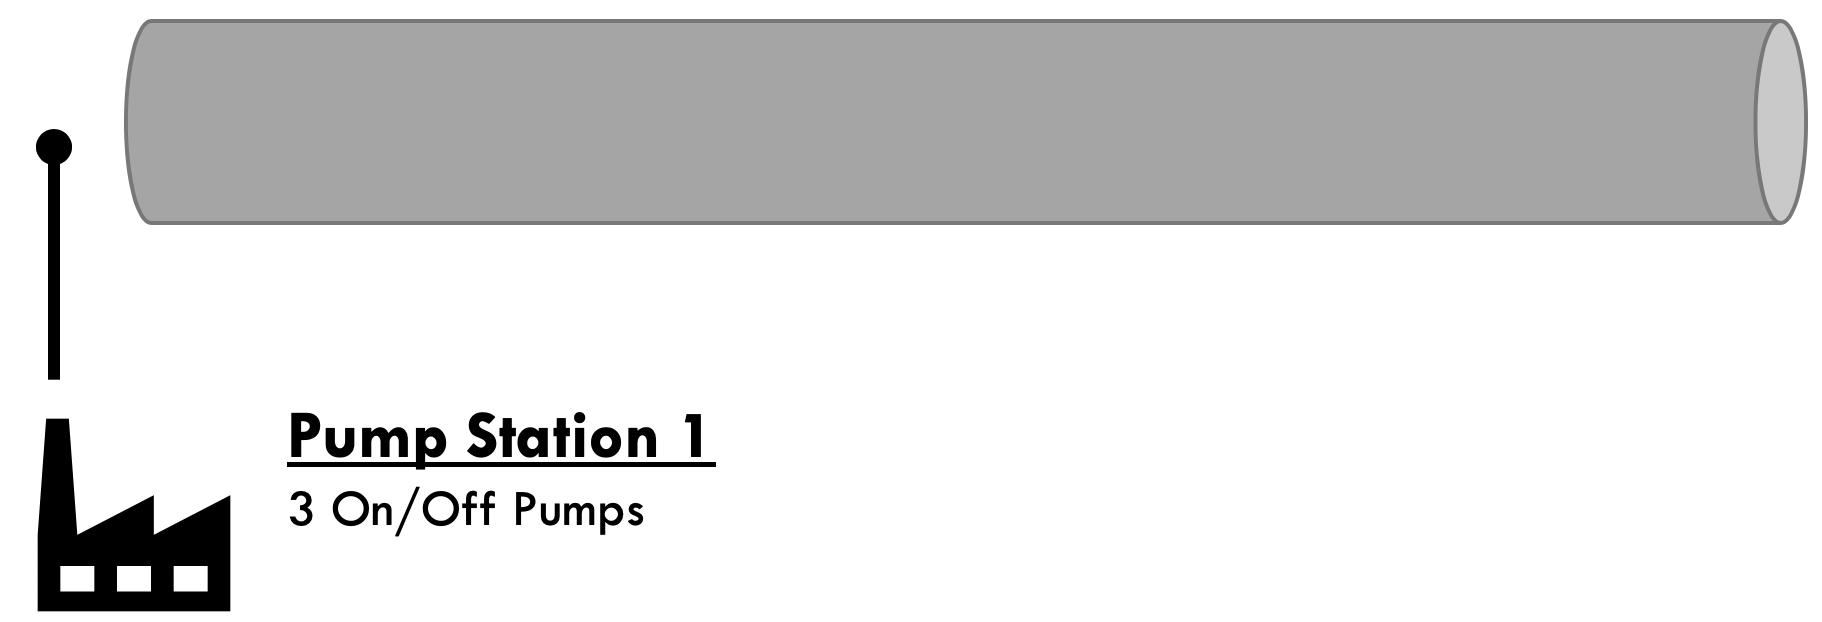
\includegraphics[scale=0.45]{images/08Line11.png}
    \caption{Schematic diagram of Line 11.}
    \label{fig:08Line11}
\end{figure}


\subsection{Line RM06A}
A schematic of line RM06A is shown in Figure \ref{fig:08RM06A}.  Line RM06A is a complex pipeline spanning 151 km and carries two products, a lighter sweet product and a heavier sour product. The two products are batched (i.e., rotate between sending each product) and each product is sent for approximately eight hours before switching to the other product. The American Petroleum Institute (API) gravity for the lighter and heavier products are roughly 40 and 20, respectively. For the rest of this chapter, the lighter and heavier product will be referred to as \textit{sweet crude} and \textit{sour crude}, respectively.

\begin{figure}[h]
    \centering
    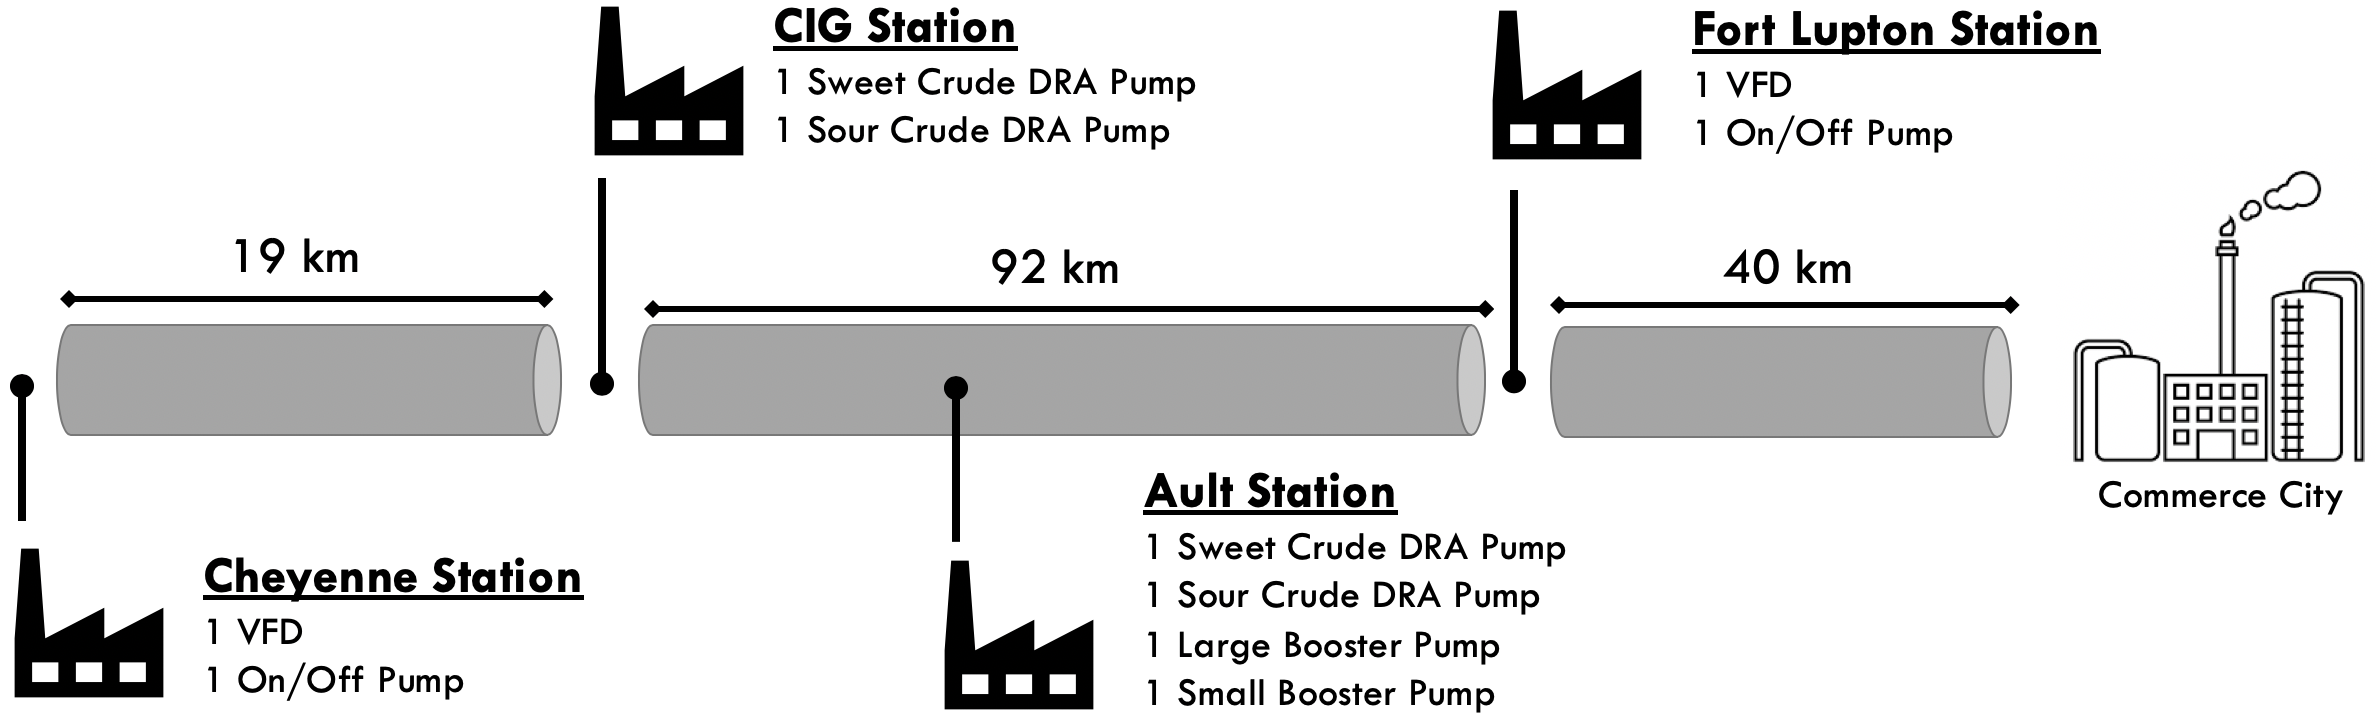
\includegraphics[scale=0.35]{images/08RM06A.png}
    \caption{Schematic diagram of Line RM06A.}
    \label{fig:08RM06A}
\end{figure}

Equipment wise, Line RM06A boasts eight pumps spread across four pump stations. Two pumps are variable frequency drives (VFD), while the rest are on/off pumps. Additionally, there are four drag reducing agent (DRA) injection pumps situated across the second and third pump stations. Each pump station contains a sour crude and sweet crude DRA pump. The sour and sweet crude uses different types of DRA and is injected based on the product present at the pump station. 



\section{Anomaly Detection}
\subsection{Data Pre-processing}
\subsection{Data Set Creation}
\subsubsection{Generative Modelling}
\subsection{Model Identification}
\subsection{Conceptual Software Design}

\section{Real Time Optimization}
Modern control systems typically consists of three layers: real time optimization (RTO), supervisory control and regulatory control.  From the top, real time optimization is evaluated the least frequently, and performs a steady state optimization of the process.  The outputs of RTO are the ideal set points for all equipment.  Next, the supervisory control layer performs dynamical optimization to identify the most efficient input trajectory to achieve the set points from RTO. Supervisory control is evaluated faster than RTO, but slower than regulatory control. Model predictive control (MPC) and economic model predictive control (EMPC) are typical supervisory control frameworks. Finally, the regulatory controllers actuate physical equipment to achieve the input trajectory given by the supervisory control layer.  Common regulatory controllers are proportional-integral-derivative (PID) controllers.

The hierarchical structure of APC is shown in Figure \ref{fig:08APC}.

\begin{figure}[h]
    \centering
    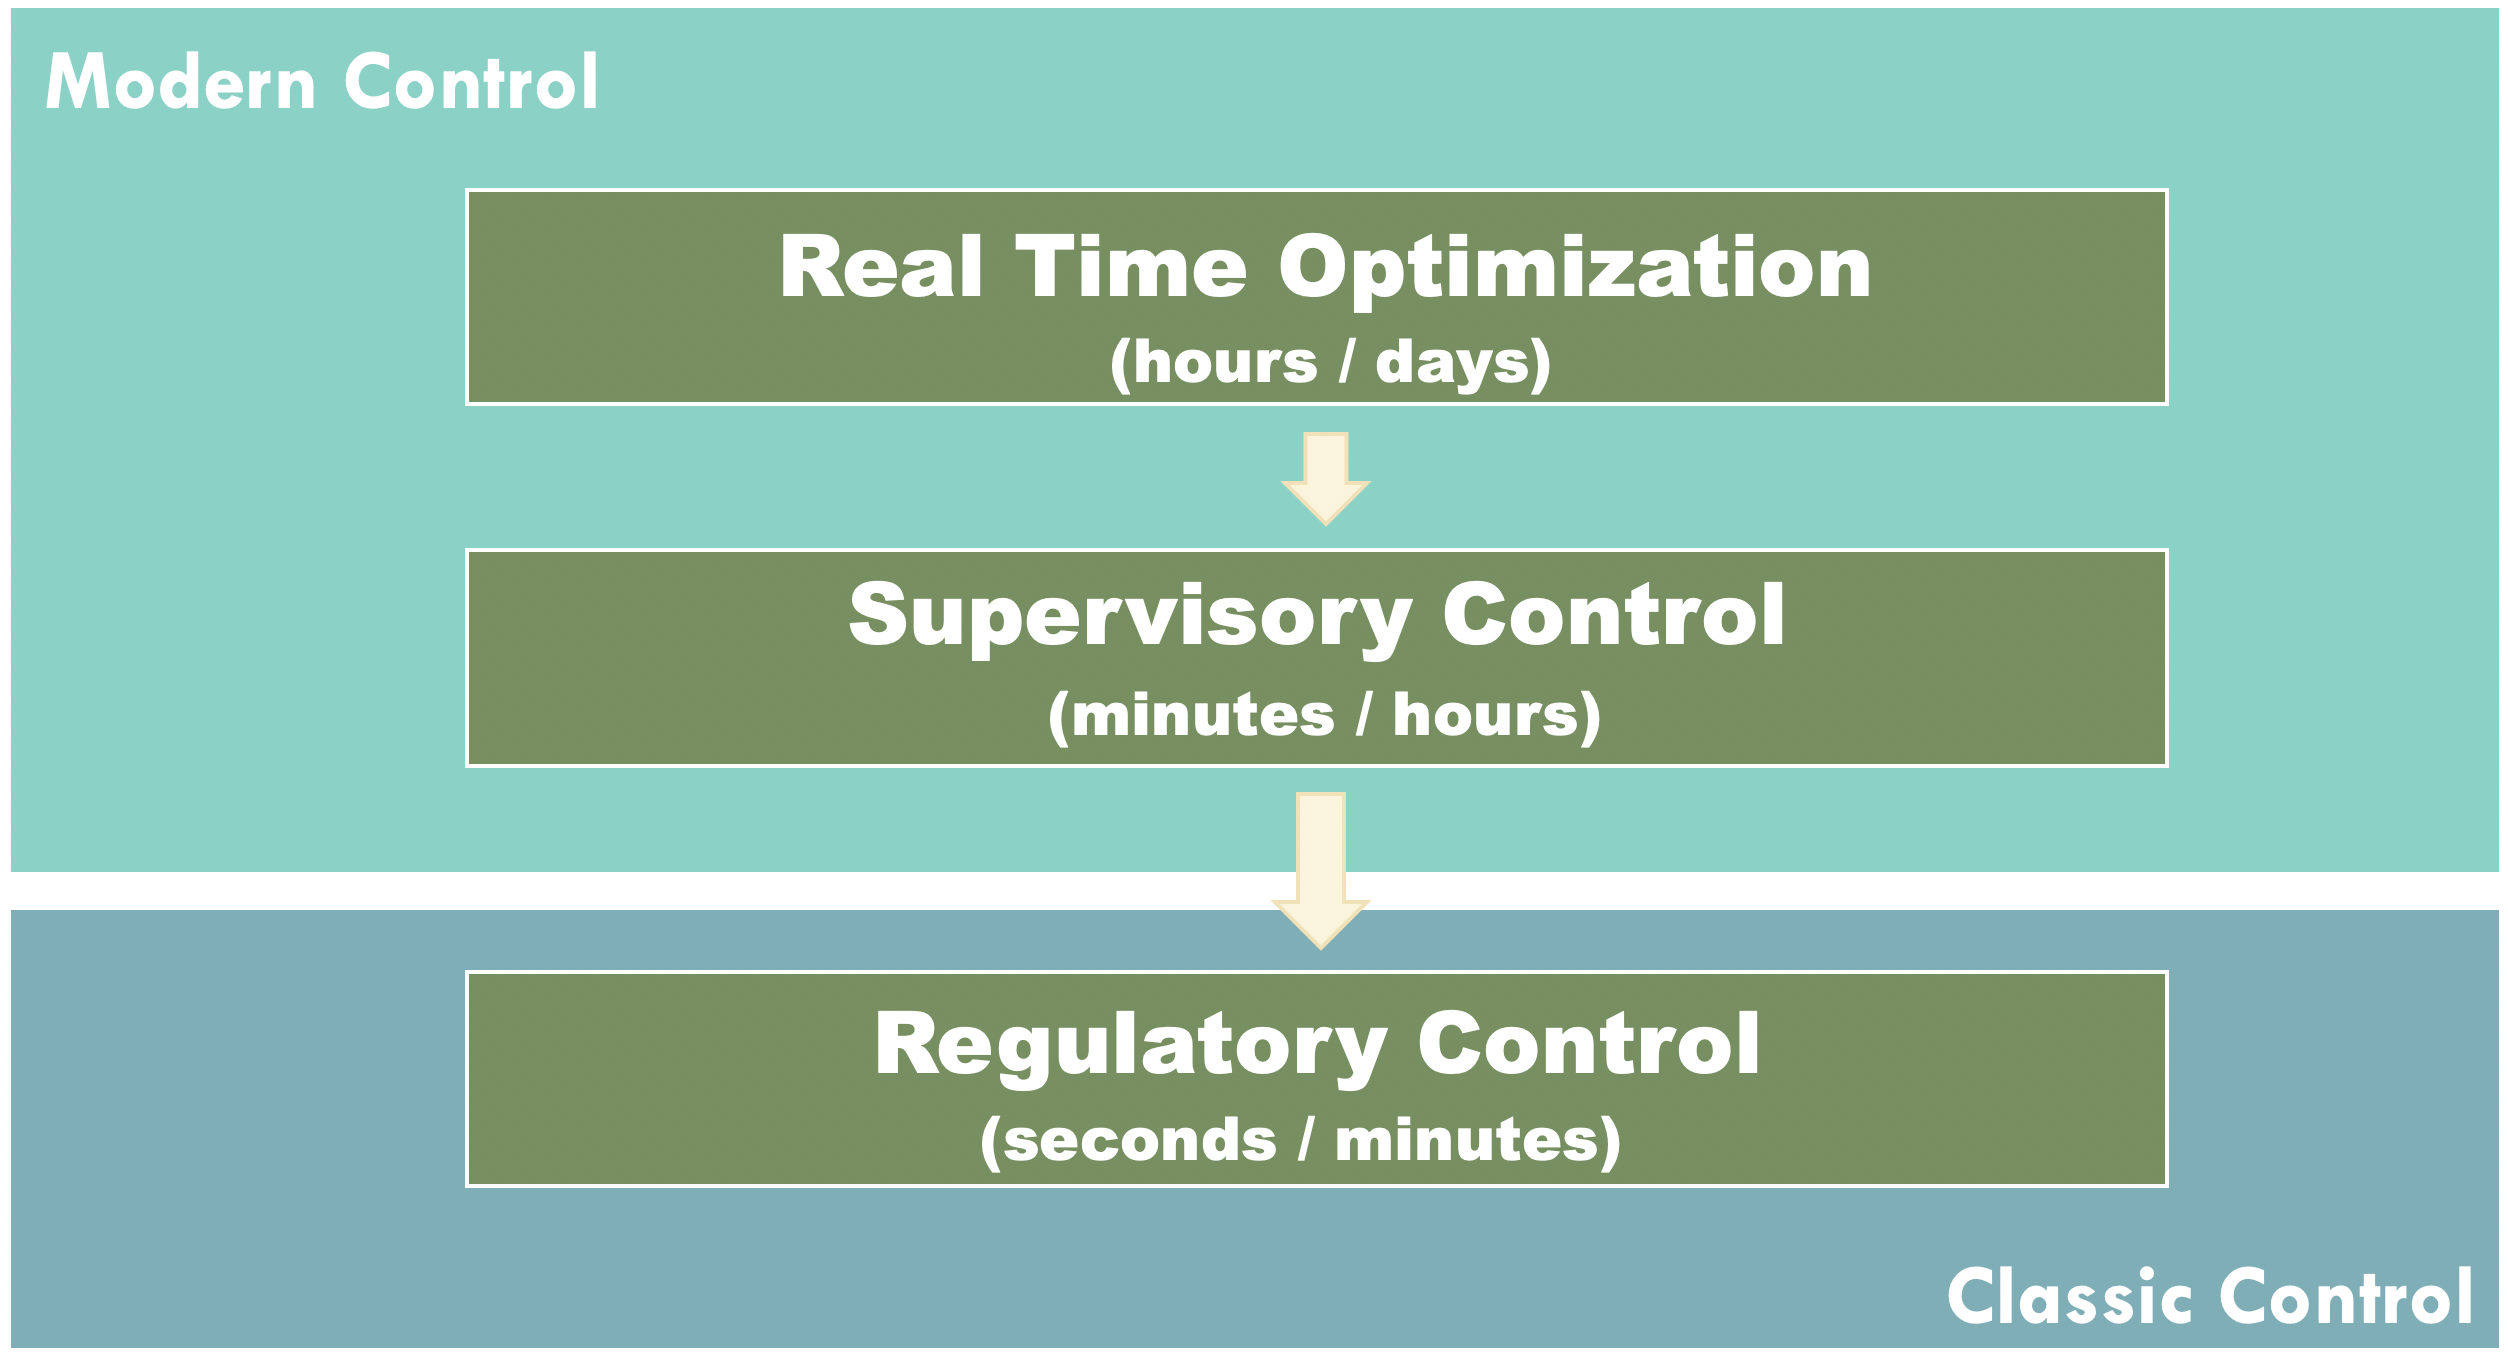
\includegraphics[scale=0.15]{images/08APC.png}
    \caption{Hierarchy of a typical modern control system.}
    \label{fig:08APC}
\end{figure}

\subsection{Problem Description}
Figure \ref{fig:08schedule} shows the communication framework of the pipeline operation. The goal of this pipeline is to meet the demands of the Commerce City refinery. To do so, a schedule with desired flow rates are sent to the operators from the scheduling team, and the operators are tasked to operate the pipeline at the given flow rate. Due to the complexity of this pipeline, different operators operate the pipeline differently even when the desired flow rate might be identical.  This difference introduces turbulence and unnecessary wear-and-tear onto the pipeline, increasing maintenance costs. 

\begin{figure}[h]
    \centering
    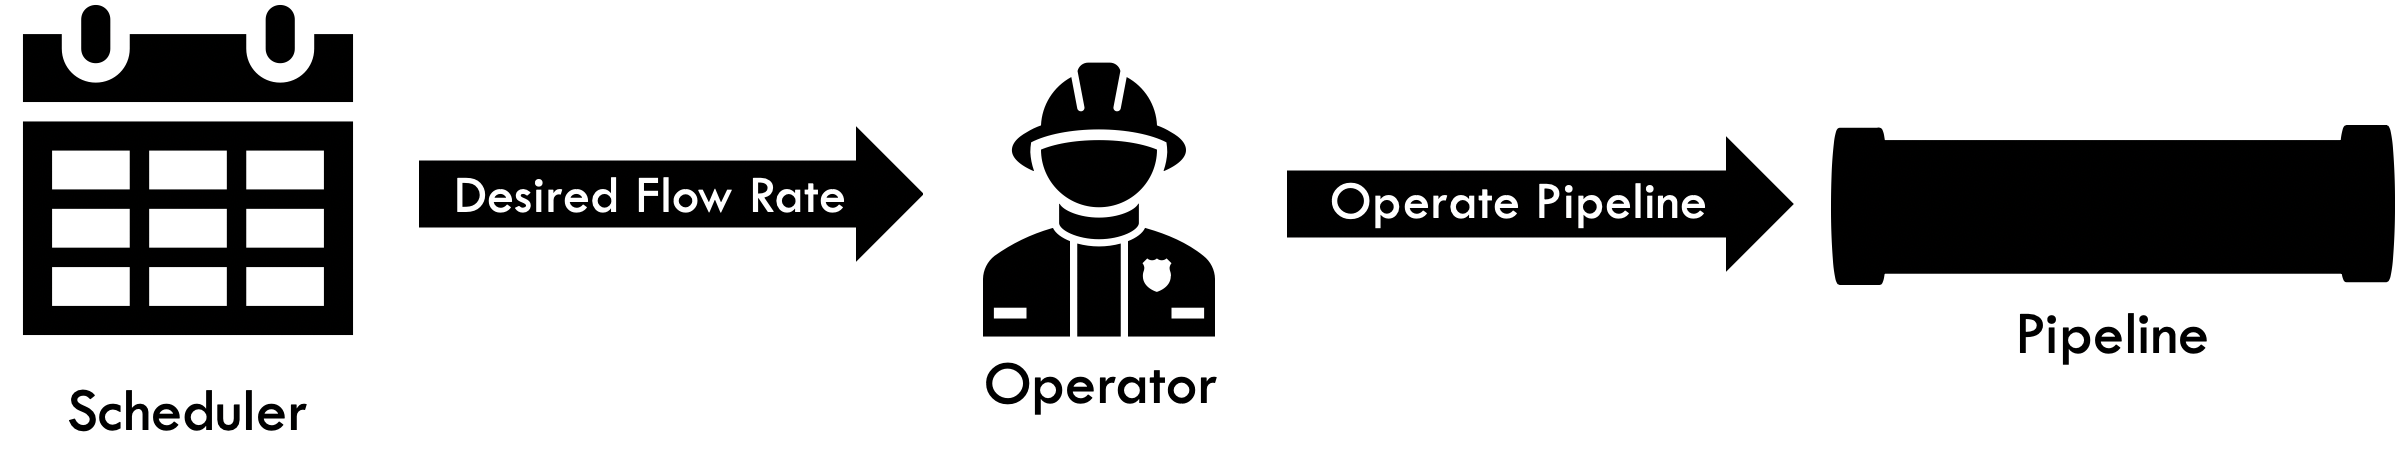
\includegraphics[scale=0.35]{images/08Schedule.png}
    \caption{Communication framework for operating line RM06A.}
    \label{fig:08schedule}
\end{figure}

To overcome this problem, machine learning was used to firstly identify a model of the pipeline.  Then, a steady state optimization tool was built using mixed integer linear programming to give operators the \textbf{optimal} set-points for each equipment.  This system solves two problems: i) Introduces uniformity in operator behaviour for desired set-points. ii) Semi-automation of the pipeline, freeing up operators' time for other tasks.

The new communication framework for line RM06A is shown in Figure \ref{fig:08scheduleV2}.

The rest of the chapters is as follows.  First, the data pre-processing step will be shown.  Then, the model identification phase will be introduced.  Following that, the optimization algorithm and all it's constraints for real-time optimization are presented.  Finally, the chapter is concluded with some conceptual software design regarding its implementation into a supervisory control and data acquisition (SCADA) system and the overall project impact will also be shown.


\begin{figure}[h]
    \centering
    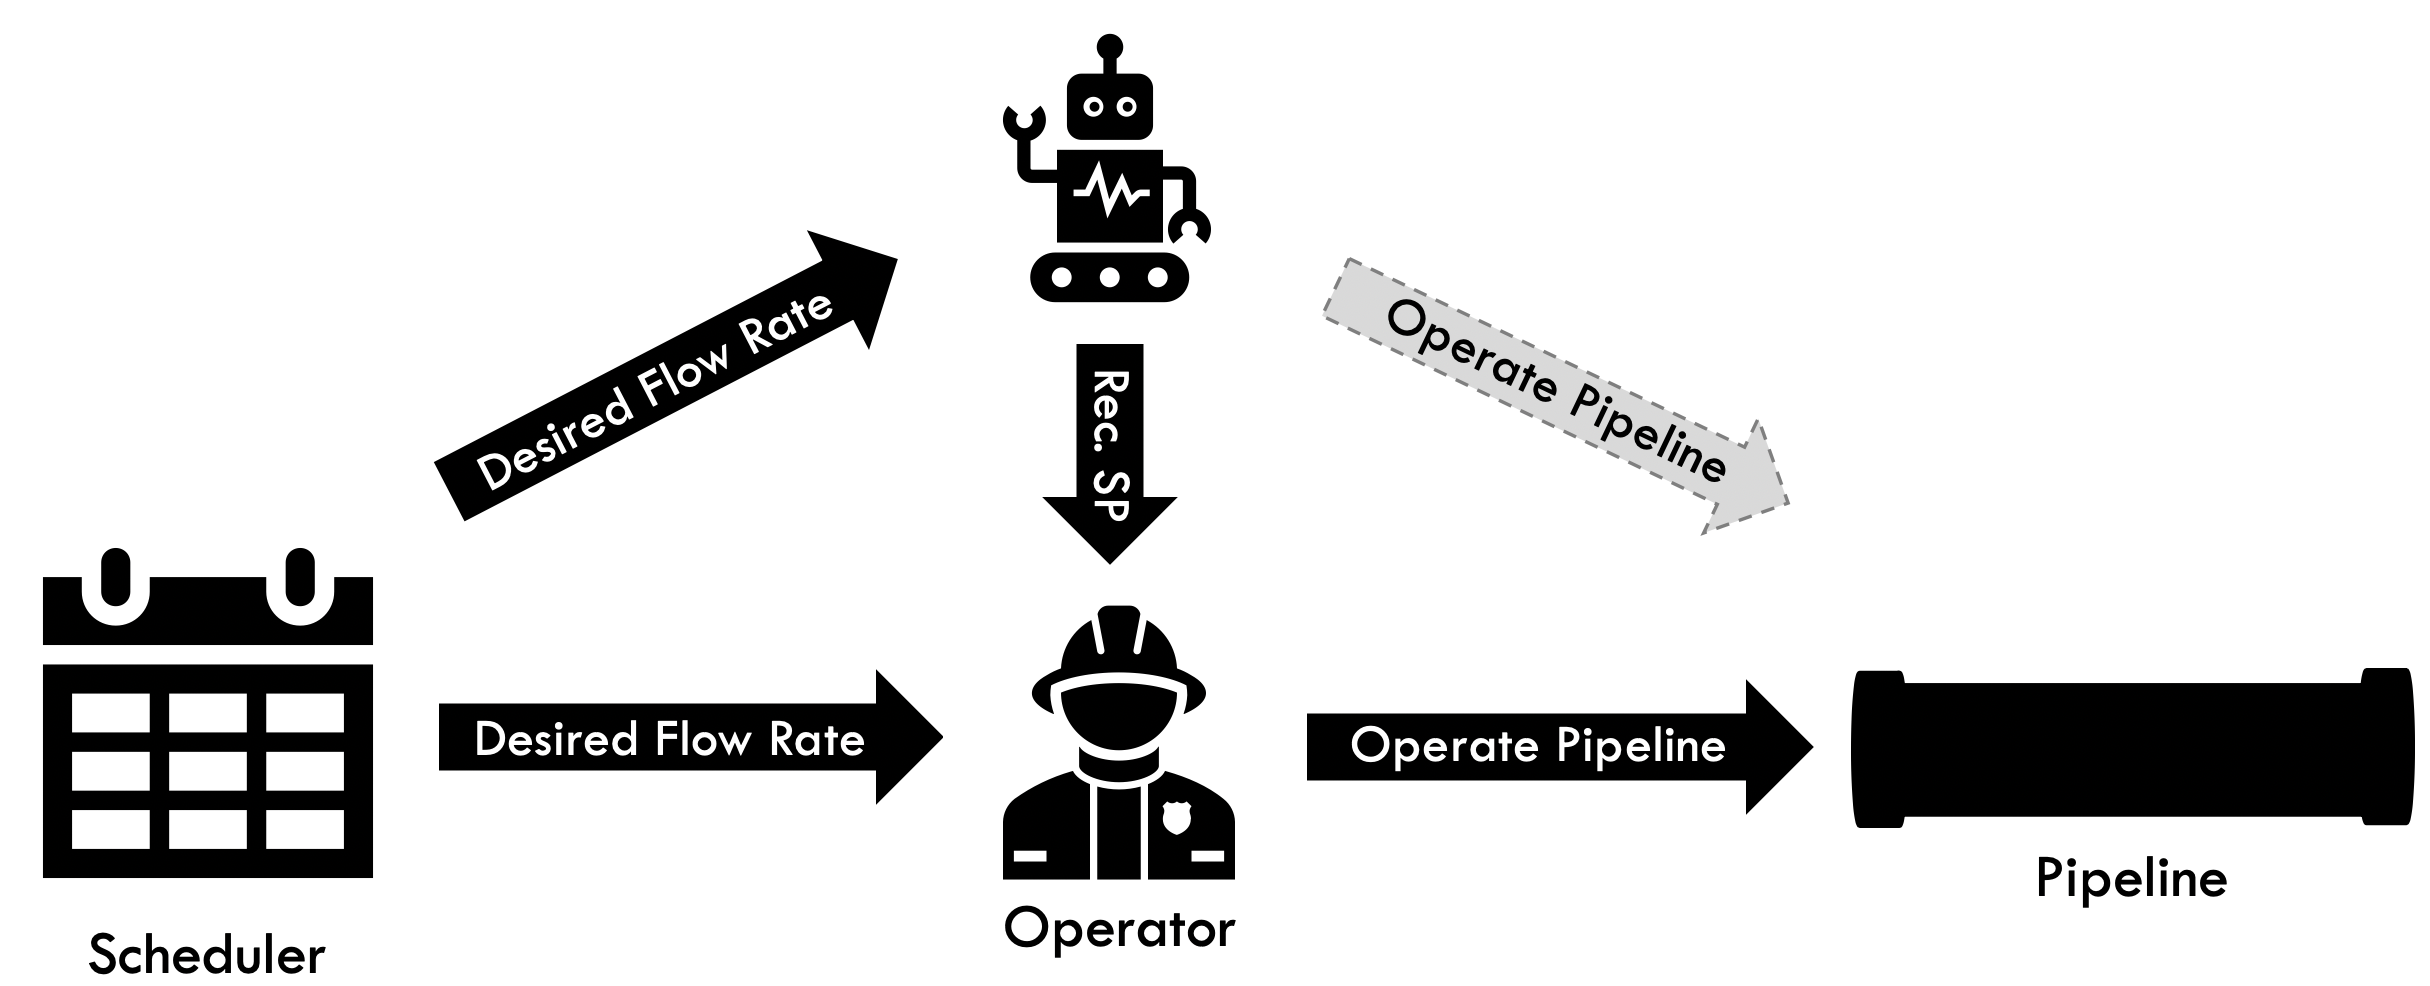
\includegraphics[scale=0.35]{images/08ScheduleV2.png}
    \caption{Proposed communication framework for operating line RM06A.}
    \label{fig:08scheduleV2}
\end{figure}

\subsection{Data Pre-processing}
Two data sets were provided by Suncor.  The details of are shown in Table \ref{tab:08data}. Model identification and optimization evaluations were conducted for both datasets; however, the steps are very similar.  Because the 2019 algorithm will go into live production, whereas the 2018 data was used as a proof of concept, only the 2019 algorithm steps will be shown in detail.

\begin{table}[h]
    \centering
    {\setstretch{1.5}
    \begin{tabular}{ c | c }
        Date of Collection     &      Data Dimension      \\
        \hline
        June 2017 - June 2018  &    $525,601 \times 899$   \\
        Dec. 2018 - March 2019 &    $159,851 \times 738$   \\
    \end{tabular}}
    \caption{Suncor data details.}
    \label{tab:08data}
\end{table}

Data pre-processing can be broken down into three phases: Filtering by subject matter experts, automated data pre-processing, and manual data pre-processing.  After the third phase, an iterative procedure followed where the subject matter experts worked alongside the machine learning scientists to give suggestions on the variables that should be included in the final model.

\subsubsection{Filtering by Subject Matter Experts}
The first phase of data pre-processing was conducted by the subject matter experts at Suncor.  The original data set contained all data corresponding to the pipeline.  Variables such as alarm limits, fire detector status, monitor on/off status, etc., have low predictive power and were removed.  After this phase, the number of variables reduced from 738 to 124.  

The distribution of the remaining variables along the pipeline can be seen in Table \ref{tab:08Ph1Data}.

\begin{table}[h]
    \centering
    {\setstretch{1.5}
    \begin{tabular}{ c | c | c | c | c | c | c}
             &  Cheyenne & CIG & Ault & Fort Lupton & Commerce City & Others      \\
        \hline
        # of Variables  &  24  &  21  &  21  &  33  &  22  &  3  \\
    \end{tabular}}
    \caption{Distribution of variables along line RM06A.}
    \label{tab:08Ph1Data}
\end{table}

\subsubsection{Automated Data Pre-processing}

\subsubsection{Manual Data Pre-processing}

\subsection{Model Identification}
\subsubsection{Feature Selection}
\subsubsection{Feature Engineering}
\subsubsection{Exploratory Modelling}
\paragraph{Linear Regression}
\paragraph{Non-linear Regression}

\subsubsection{Model Structure}
Ultimately, a linear parameter-varying (LPV) model was selected to model this pipeline.  It is clear that the process is heavily non-linear due to the increase in accuracy when switching to a non-linear model structure; therefore, LPV models were selected due to their non-linear nature while still retaining the interpretability of linear models. To enhance credibility, any non-linear model can be approximated by a LPV model via the White's Theorem \cite{LPV}.

\subsection{Mixed Integer Linear Programming}
\subsection{Conceptual Software Design}
\subsection{Cost Savings and Impact on Society}
